\documentclass{standalone}

\usepackage{tikz}

\begin{document}
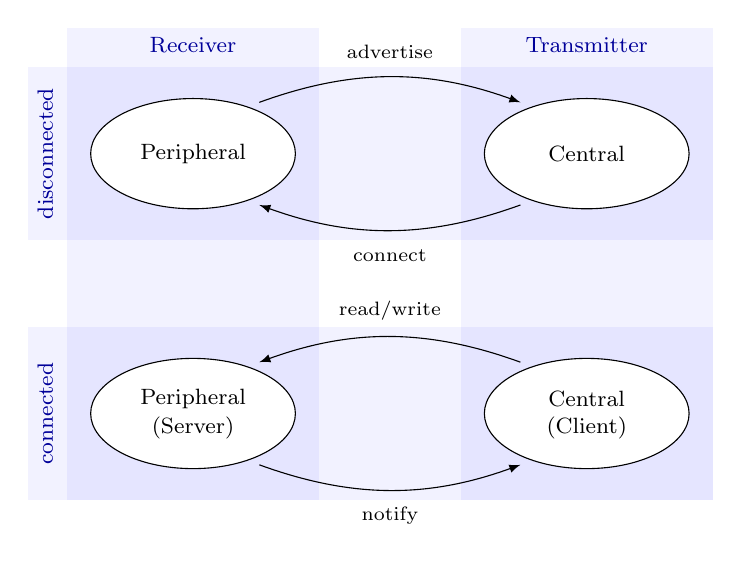
\begin{tikzpicture}
	\tikzset{
	state/.style={circle,draw,minimum size=6ex},
	arrow/.style={-latex, shorten >=1ex, shorten <=1ex}}

	\def\sh{3.3};

	

	\fill[blue!5!white] (-1.6,1.6) rectangle (1.6,-1.1-\sh);
	\fill[blue!5!white] (-1.6+5,1.6) rectangle (1.6+5,-1.1-\sh);

	\fill[blue!5!white] (-2.1,1.1) rectangle (5+1.2,-1.1);
	\fill[blue!5!white] (-2.1,1.1-\sh) rectangle (5+1.2,-1.1-\sh);
	
	\fill[blue!10!white] (-1.6,1.1) rectangle (1.6,-1.1);
	\fill[blue!10!white] (-1.6,1.1-\sh) rectangle (1.6,-1.1-\sh);
	\fill[blue!10!white] (-1.6+5,1.1) rectangle (1.6+5,-1.1);
	\fill[blue!10!white] (-1.6+5,1.1-\sh) rectangle (1.6+5,-1.1-\sh);

	\node[below, blue!60!black] at (0,1.6) {\footnotesize Receiver};
	\node[below, blue!60!black] at (5,1.6) {\footnotesize Transmitter};

	\node[rotate=90, below, blue!60!black] at (-2.1,0) {\footnotesize disconnected};
	\node[rotate=90, below, blue!60!black] at (-2.1,0-\sh) {\footnotesize connected};

	%disconnected
	\fill[white, draw=black] (0,0) ellipse (1.3 and 0.7);
	\node at (0,0) {\footnotesize Peripheral};
	\fill[white, draw=black] (5,0) ellipse (1.3 and 0.7);
	\node at (5,0) {\footnotesize Central};
		
	\draw [arrow, bend left=20] (0.7,0.6) to (4.3,0.6);
	\draw [arrow, bend left=20] (4.3,-0.6) to (0.7,-0.6);
	\node at (2.5,1.3) {\scriptsize advertise};
	\node at (2.5,-1.3) {\scriptsize connect};
		
	%connected	
	\fill[white, draw=black] (0,0-\sh) ellipse (1.3 and 0.7);
	\node at (0,0.19-\sh) {\footnotesize Peripheral};
	\node at (0,-0.19-\sh) {\footnotesize (Server)};
	\fill[white, draw=black] (5,0-\sh) ellipse (1.3 and 0.7);
	\node at (5,0.19-\sh) {\footnotesize Central};
	\node at (5,-0.19-\sh) {\footnotesize (Client)};
		
	\draw [arrow, bend right=20] (4.3,0.6-\sh) to (0.7,0.6-\sh);
	\draw [arrow, bend right=20] (0.7,-0.6-\sh) to (4.3,-0.6-\sh);
	
	\node at (2.5,1.3-\sh) {\scriptsize read/write};
	\node at (2.5,-1.3-\sh) {\scriptsize notify};
		
\end{tikzpicture}		
\end{document}